\documentclass[tikz,border=3mm]{standalone}
\usepackage{tikz}
\usetikzlibrary{angles,quotes,calc,intersections}
\begin{document}
% TikZ 1
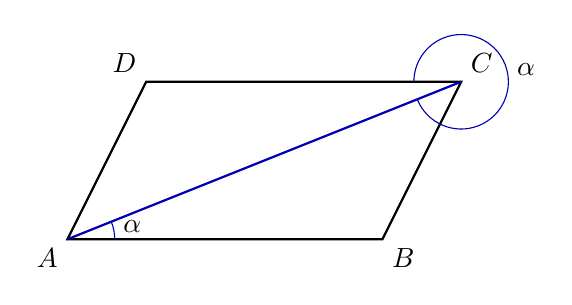
\begin{tikzpicture}[scale=1]
\coordinate (A) at (0,0); \coordinate (B) at (4,0); \coordinate (C) at (5,2); \coordinate (D) at (1,2);
\draw[thick] (A)--(B)--(C)--(D)--cycle;
\draw[blue!70!black,thick] (A)--(C);
\pic[draw=blue!70!black, "$\alpha$", angle radius=6mm, angle eccentricity=1.4] {angle=B--A--C};
\pic[draw=blue!70!black, "$\alpha$", angle radius=6mm, angle eccentricity=1.4] {angle=A--C--D};
\foreach \p/\pos in {A/below left,B/below right,C/above right,D/above left}{\node[\pos] at (\p) {$\p$};}
\end{tikzpicture}
\hspace{1cm}
% TikZ 2
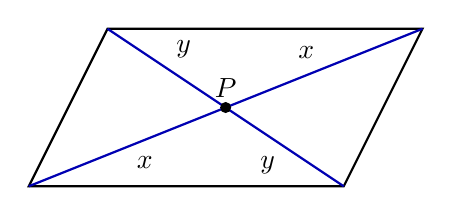
\begin{tikzpicture}[scale=1]
\coordinate (A) at (0,0); \coordinate (B) at (4,0); \coordinate (C) at (5,2); \coordinate (D) at (1,2);
\coordinate (P) at ($(A)!0.5!(C)$);
\draw[thick] (A)--(B)--(C)--(D)--cycle;
\draw[blue!70!black,thick] (A)--(C);
\draw[blue!70!black,thick] (B)--(D);
\fill (P) circle (2pt);
\node[above] at (P) {$P$};
\node[below right] at ($(A)!0.5!(P)$) {$x$};
\node[above left] at ($(P)!0.5!(C)$) {$x$};
\node[below left] at ($(B)!0.5!(P)$) {$y$};
\node[above right] at ($(P)!0.5!(D)$) {$y$};
\end{tikzpicture}

\vspace{1cm}

% TikZ 3
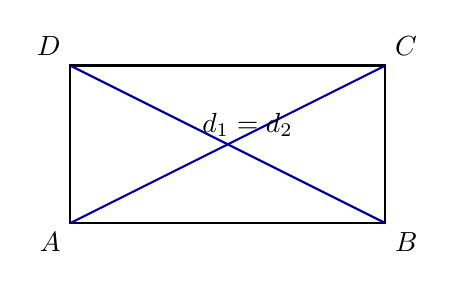
\begin{tikzpicture}[scale=1]
\coordinate (A) at (0,0); \coordinate (B) at (4,0); \coordinate (C) at (4,2); \coordinate (D) at (0,2);
\draw[thick] (A)--(B)--(C)--(D)--cycle;
\draw[blue!70!black,thick] (A)--(C);
\draw[blue!70!black,thick] (B)--(D);
\node at (2.25,1.25) {$d_1=d_2$};
\foreach \p/\pos in {A/below left,B/below right,C/above right,D/above left}{\node[\pos] at (\p) {$\p$};}
\end{tikzpicture}
\hspace{1cm}
% TikZ 4
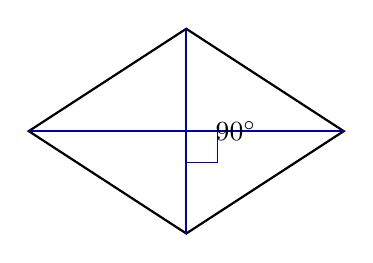
\begin{tikzpicture}[scale=1]
\coordinate (A) at (0,0); \coordinate (B) at (2,1.3); \coordinate (C) at (0,2.6); \coordinate (D) at (-2,1.3);
\coordinate (P) at (0,1.3);
\draw[thick] (A)--(B)--(C)--(D)--cycle;
\draw[blue!70!black,thick] (A)--(C);
\draw[blue!70!black,thick] (B)--(D);
\pic[draw=blue!70!black, angle radius=4mm] {right angle=A--P--B};
\node[right] at (.25,1.3) {$90^{\circ}$};
\end{tikzpicture}

\vspace{1cm}

% TikZ 5
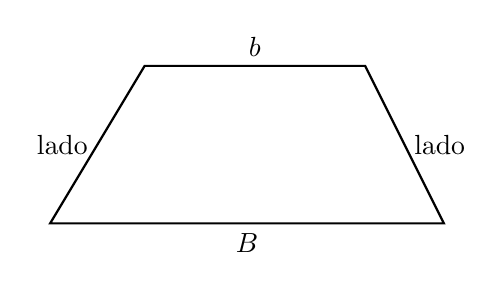
\begin{tikzpicture}[scale=1]
\coordinate (A) at (0,0); \coordinate (B) at (5,0); \coordinate (C) at (4,2); \coordinate (D) at (1.2,2);
\draw[thick] (A)--(B)--(C)--(D)--cycle;
\node[below] at ($(A)!0.5!(B)$) {$B$};
\node[above] at ($(D)!0.5!(C)$) {$b$};
\node[left] at ($(A)!0.5!(D)$) {lado};
\node[right] at ($(B)!0.5!(C)$) {lado};
\end{tikzpicture}
\hspace{1cm}
% TikZ 6
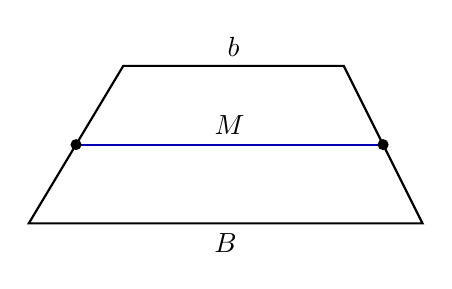
\begin{tikzpicture}[scale=1]
\coordinate (A) at (0,0); \coordinate (B) at (5,0); \coordinate (C) at (4,2); \coordinate (D) at (1.2,2);
\coordinate (E) at ($(A)!0.5!(D)$); \coordinate (F) at ($(B)!0.5!(C)$);
\draw[thick] (A)--(B)--(C)--(D)--cycle;
\draw[blue!70!black,thick] (E)--(F);
\fill (E) circle (2pt); \fill (F) circle (2pt);
\node[below] at ($(A)!0.5!(B)$) {$B$};
\node[above] at ($(D)!0.5!(C)$) {$b$};
\node[above] at ($(E)!0.5!(F)$) {$M$};
\end{tikzpicture}
\end{document}
